\section{Problem Formulation}
% 在铝合金锻造过程中，位移场、温度场与应力场构成高度耦合的非线性动力学系统。温度场作为关键状态变量，主导材料本构响应：高温能够软化材料、降低流动应力，低温则导致材料硬化与变形抗力增大。预热工序将坯料加热至固定始锻温度，故不作为实时决策量。锻造速度作为核心控制变量，通过改变应变速率影响应力场：速率过高引发应变率强化，应力剧增导致开裂风险；速率过低则延长锻压时间，坯料温降增大变形抗力，同样加剧开裂。

% 因此，本研究将锻造速度决策问题建模为式\eqref{equ:model}所示的优化问题：
% \begin{equation}
% \begin{split}
% \min_{v_{y}(t)} f(t_f)  \, \text{subject to} & \, \int_{0}^{t_f} v_{y}(t) \, dt = \Delta h = \text{const} \\
% \max C(t) &< C_{\text{cr}} \quad \forall t \in [0, t_f]
% \end{split}
% \label{equ:model}
% \end{equation}

% 目标是在恒定锻压行程 $\Delta h$ 下寻求最优速度曲线 $v_y(t)$，以最短时间 $t_f$ 完成锻造，并确保损伤 $D(t)$ 始终低于临界值 $D_{\text{cr}}$，从而平衡生产效率与质量。



% 为实现上述目标，本文的研究路径包含以下两个核心阶段，整体流程如图\ref{fig:frame}所示：
% % \begin{figure*}[htbp]
% % \centerline{\includegraphics[width=\textwidth]{frame.pdf}}
% % \caption{Example of a figure caption.}
% % \label{fig:frame}
% % \end{figure*}

% \begin{figure}[htbp]
% \centerline{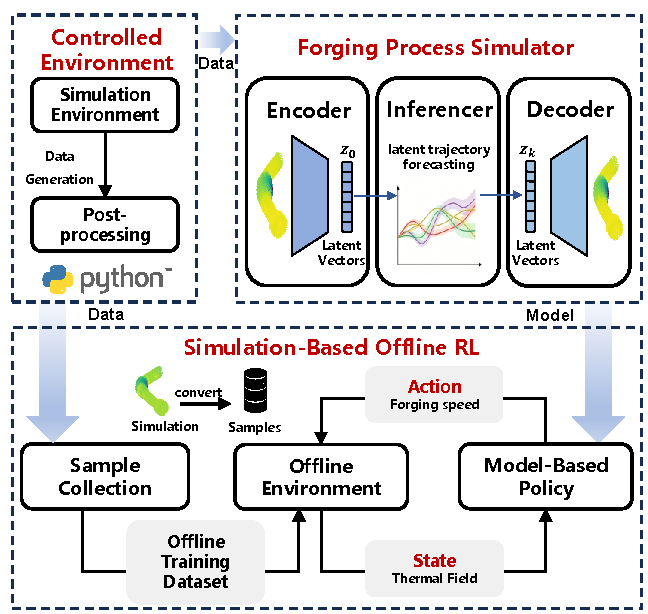
\includegraphics[width=\linewidth]{frame-1.pdf}}
% \caption{The framework of research .}
% \label{fig:frame}
% \end{figure}

% \begin{enumerate}
%     \item \textbf{代理模型构建}：基于Deform仿真数据训练DeepONet代理模型，实现从初始温度场和速度曲线到多物理场演化的端到端快速预测。
%     \item \textbf{控制策略优化}：在代理模型构成的虚拟环境中，采用离线强化学习训练决策网络，根据初始状态生成最优速度参数，同步优化质量与效率。
% \end{enumerate}
The aluminum alloy forging process constitutes a highly coupled,
nonlinear dynamic system involving displacement, temperature, and stress
fields. The temperature field, a key state variable, governs the
material's constitutive response: elevated temperatures soften the
material and reduce flow stress, while lower temperatures cause
hardening and increase deformation resistance. The initial billet is
heated to a fixed start-forging temperature, which is thus not a
real-time decision variable. The forging speed, as the core control
variable, influences the stress field by altering the strain rate.
Excessively high speeds induce strain-rate hardening, sharply increasing
stress and cracking risk; excessively low speeds prolong the process,
leading to significant temperature drop and increased deformation
resistance, which also elevates the risk of cracking.

Consequently, the forging speed decision is formulated as the
optimization problem in Eq. \eqref{equ:model}:
\begin{equation}
\begin{split}
\min_{v_{y}(t)} f(t_f) \, \text{subject to} & \, \int_{0}^{t_f} v_{y}(t) \, dt = \Delta h = \text{const} \\
D(t) &< D_{\text{cr}} \quad \forall t \in [0, t_f]
\end{split}
\label{equ:model}
\end{equation}
The objective is to determine an optimal speed curve $v_y(t)$ for a
constant forging stroke $\Delta h$ that minimizes the total time $t_f$,
while ensuring the damage indicator $D(t)$ remains below a critical
threshold $D_{\text{cr}}$ throughout the process, thereby balancing
productivity and quality.

The research pathway to achieve this objective comprises two core
stages, as illustrated in Fig. \ref{fig:frame}:
\begin{enumerate}
    \item \textbf{Surrogate Model Construction}: A DeepONet is trained
    on data from Deform simulations to enable fast, end-to-end
    prediction of multi-physics field evolution from initial temperature
    fields and speed profiles.
    \item \textbf{Control Policy Optimization}: An offline reinforcement
    learning agent is trained within the virtual environment provided by
    the surrogate model. This agent generates optimal speed parameters
    based on the initial state, simultaneously optimizing both quality
    and efficiency.
\end{enumerate}
